\documentclass{article}                          %%%定义文档类型
\usepackage[utf8]{inputenc}
\usepackage{ctex}                                %%%中文支持
\usepackage{amsmath}                             %%%数学公式包
\numberwithin{equation}{subsection}              %%%公式自动编号
\usepackage{geometry}
\geometry{left=0.95in,right=0.95in,top=1in,bottom=1in}
\usepackage{graphicx}                            %%%图片支持
\usepackage{caption}
\title{对于高斯积分中坐标变换的理解-1D}
\author{李晓东,中国地质大学(武汉)工程学院}
\begin{document}
\maketitle
\section{ 高斯积分公式}
对于这样的一个一维积分:
\begin{equation}\label{key}
\int_{a}^{b} f(t) dt
\end{equation}
必须把它的上下限转化到(-1,1)区间,才能直接使用高斯-勒让德求积公式。
为此寻找如下线性变换:
\begin{equation}\label{key}
c_1 x+c_2=t
\end{equation}
分别代入积分上下限,可以得到:
\begin{equation}\label{key}
\begin{aligned}
&c_1+c_2=b\\
-&c_1+c_2=a\\
\end{aligned}
\end{equation}
求解之后可以得到:
\begin{equation}\label{key}
\begin{aligned}
&c_1=\frac{b-a}{2}\\
&c_2=\frac{a+b}{2}
\end{aligned}
\end{equation}
所以变换关系为:
\begin{equation}\label{key}
t=\frac{b-a}{2} x+ \frac{a+b}{2}
\end{equation}
最终可以直接使用的积分公式变为:
\begin{equation}\label{key}
\int_{a}^{b} f(t) dt= \frac{b-a}{2} \int_{-1}^{1} f\left(\frac{b-a}{2} x+ \frac{a+b}{2} \right) dx
\end{equation}
这样对于一个具体的积分,我们只需要知道$ a,b,$ and $f $,然后利用下式,即可计算积分值:
\begin{equation}\label{key}
\int_{a}^{b} f(t) dt= \frac{b-a}{2} \sum_{i=0}^{N} A_i f\left(\frac{b-a}{2} x_i+ \frac{a+b}{2} \right)
\end{equation}
\begin{figure}
	\centering
	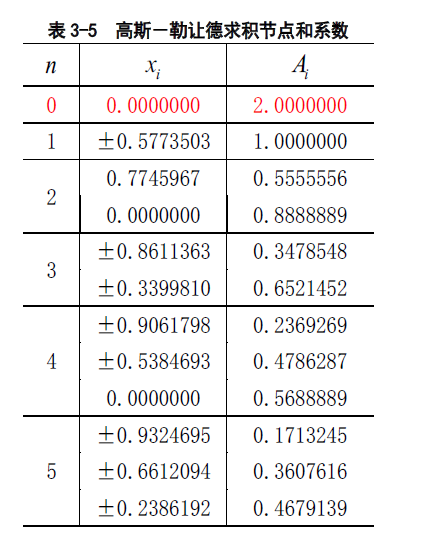
\includegraphics{xishu.png}
\end{figure}
\section{算例}
1、使用高斯-勒让德求积公式计算:
\begin{equation}\label{key}
\int_{0}^{\frac{\pi}{2}}x^2 \cos x dx
\end{equation}
为了简单直观,我们使用Wolfram mathematica计算上述积分,具体计算过程由图\ref{fig1}给出。\\
\begin{figure}
	\centering
	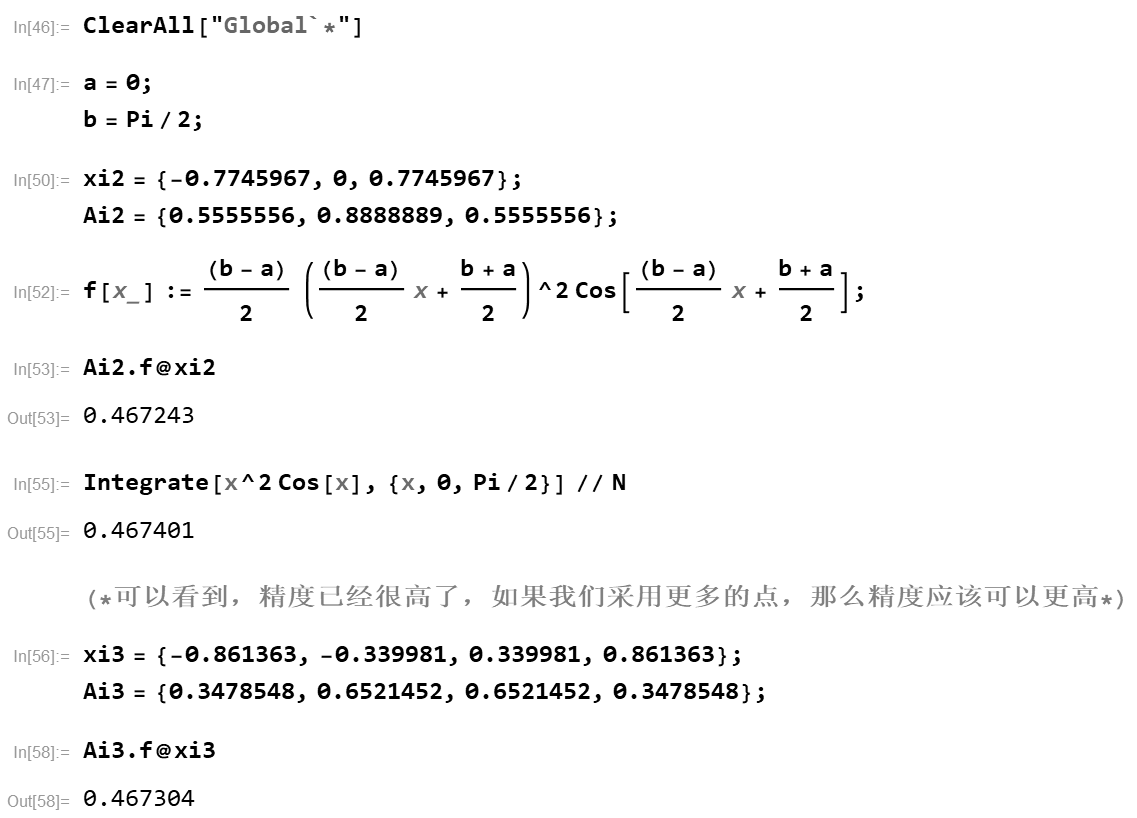
\includegraphics[width=\linewidth]{高斯积分公式的计算.png}
	\caption{Wolfram mathematica计算高斯积分的过程}
	\label{fig1}
\end{figure}
可以看到使用该高斯积分公式可以在使用几个点的情况下就可以达到比较高的精度,完全可以满足实际计算的需要。\\
2:使用高斯-勒让德求积公式计算:
\begin{equation}\label{key}
\int_{2}^{4}\ln(x) dx
\end{equation}
计算过程如图\ref{fig2}所示
\begin{figure}[h]
		\centering
	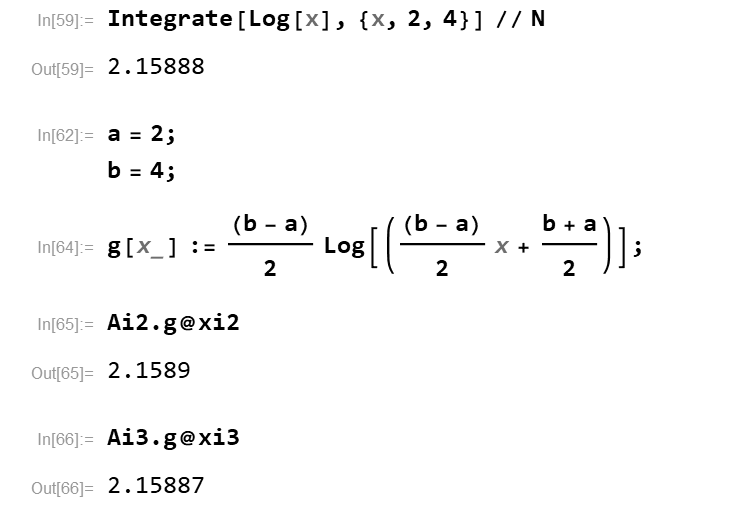
\includegraphics[width=\linewidth]{lnx.png}
	\caption{Wolfram mathematica计算$ \int_{2}^{4}\ln(x) $的过程}
	\label{fig2}
\end{figure}

3:使用高斯-勒让德求积公式计算:
\begin{equation}\label{key}
\int_{1}^{10}\sin(x) dx
\end{equation}
计算过程如图\ref{fig3}所示
\begin{figure}[h]
	\centering
	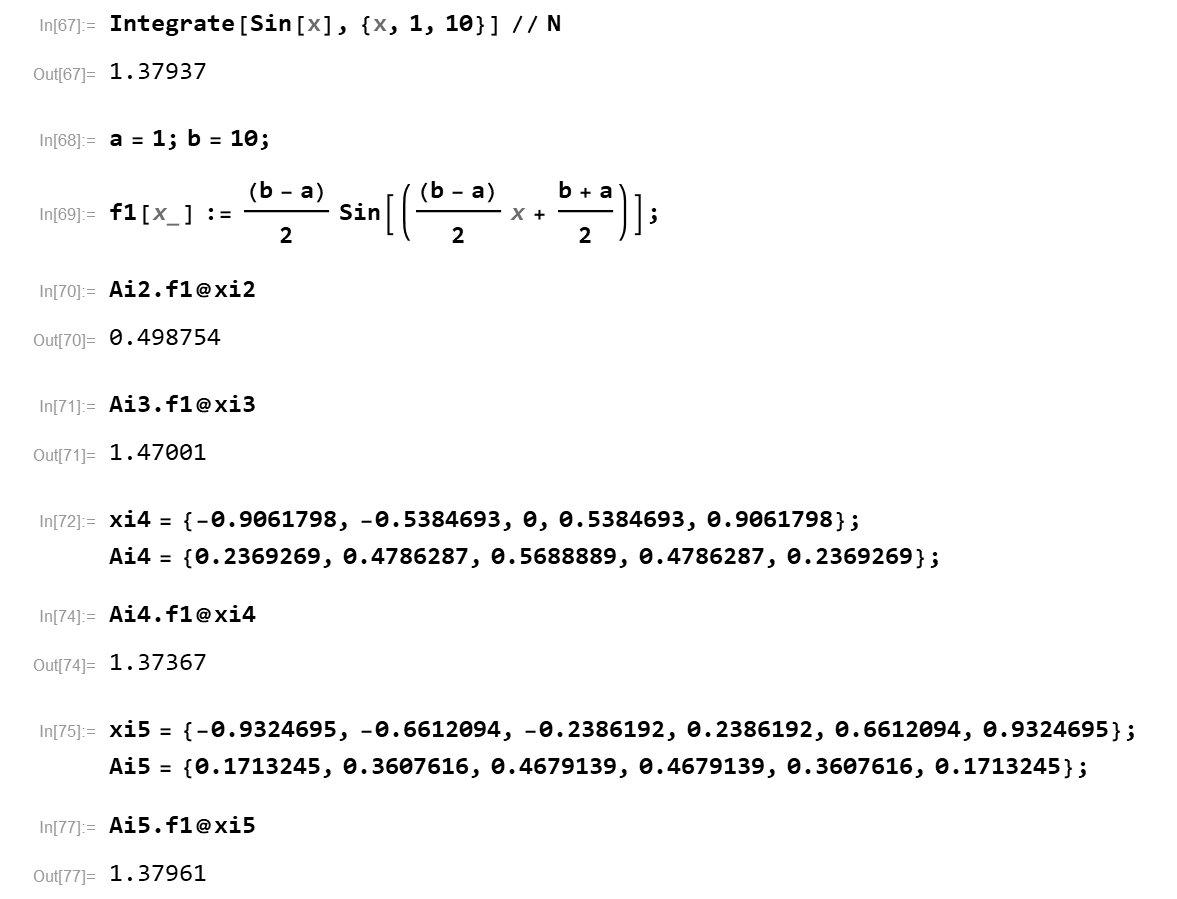
\includegraphics[width=\linewidth]{sinx1_10.png}
	\caption{Wolfram mathematica计算$\int_{1}^{10}\sin(x) dx $的过程}
	\label{fig3}
\end{figure}
可以看到,该积分需要使用更多的节点,才能达到比较高的精度。
\end{document}